%% ============================================================================
%%  NATURE ASTRONOMY — ARTICLE SUBMISSION
%%
%%  Title: Holographic Resolution of the Hubble Tension: A Six-Dataset,
%%         First-Principles Determination of the Cosmological Constant
%%         from Galaxy Rotation Curves to the CMB Power Spectrum
%%
%%  Author: Kevin Henry Miller
%%  Affiliation: Q-Bond Network DeSCI DAO, LLC
%%
%%  Compile: pdflatex main_manuscript.tex (twice)
%% ============================================================================

\documentclass[12pt,a4paper]{article}

%% -- Packages -----------------------------------------------------------------
\usepackage[margin=2.5cm]{geometry}
\usepackage{amsmath,amssymb,amsthm}
\usepackage{graphicx}
\usepackage{booktabs}
\usepackage{multirow}
\usepackage{setspace}
\usepackage{fancyhdr}
\usepackage{titlesec}
\usepackage{caption}
\usepackage{subcaption}
\usepackage{enumitem}
\usepackage{xcolor}
\usepackage{microtype}
\usepackage{array}
\usepackage{lmodern}
\usepackage[T1]{fontenc}
\usepackage[numbers,sort&compress]{natbib}
\usepackage[colorlinks=true,linkcolor=blue!70!black,
            citecolor=green!50!black,urlcolor=blue!60!black]{hyperref}
\usepackage{lineno}
\usepackage{parskip}
\graphicspath{{figures/}}

%% -- Line spacing and numbering (required for peer review) -------------------
\setstretch{1.5}
\linenumbers

%% -- Header/footer -----------------------------------------------------------
\pagestyle{fancy}
\fancyhf{}
\rhead{\footnotesize \textit{Nature Astronomy --- Manuscript}}
\lhead{\footnotesize \textit{Miller --- Holographic Cosmological Constant}}
\cfoot{\thepage}

%% -- Section formatting ------------------------------------------------------
\titleformat{\section}{\normalfont\bfseries\large}{\thesection}{1em}{}
\titleformat{\subsection}{\normalfont\bfseries\normalsize}{\thesubsection}{1em}{}

%% -- Custom commands ---------------------------------------------------------
\newcommand{\lcdm}{$\Lambda$CDM}
\newcommand{\OmL}{\Omega_\Lambda}
\newcommand{\Omm}{\Omega_m}
\newcommand{\lP}{l_\mathrm{P}}
\newcommand{\rH}{r_\mathrm{H}}
\newcommand{\rhocrit}{\rho_\mathrm{crit}}
\newcommand{\rhoP}{\rho_\mathrm{P}}
\newcommand{\kms}{\,\mathrm{km\,s^{-1}\,Mpc^{-1}}}
\newcommand{\msq}{\,\mathrm{m}^{-2}}
\newcommand{\Qal}{Q_{\mathrm{align}}}

%% ============================================================================
\begin{document}

\noindent{\Large\bfseries
Holographic Resolution of the Hubble Tension: A Six-Dataset,
First-Principles Determination of the Cosmological Constant
from Galaxy Rotation Curves to the CMB Power Spectrum}

\vspace{0.8cm}
\noindent
\textbf{Kevin Henry Miller}$^{1,*}$

\vspace{0.3cm}
\noindent
$^1$Q-Bond Network DeSCI DAO, LLC, 965 Garnet Drive, Acworth, Georgia 30101, USA

\vspace{0.2cm}
\noindent
$^*$Correspondence: Kevin@qbondnetwork.com $\;\cdot\;$ ORCID: 0009-0007-7286-3373

\vspace{0.5cm}
\noindent\textbf{Received:} March 3, 2026 $\;\cdot\;$ \textbf{Submitted to:} \textit{Nature Astronomy}

\vspace{0.8cm}
\noindent\rule{\linewidth}{0.5pt}

%% ============================================================================
%% ABSTRACT
%% ============================================================================

\begin{center}{\large\bfseries Abstract}\end{center}

\noindent
The Hubble tension---a discrepancy of 4--6$\sigma$ between early-universe
($H_0 = 67.4 \pm 0.5\kms$, Planck 2018) and late-universe
($H_0 = 73.0 \pm 1.0\kms$, SH0ES) determinations of the Hubble constant---
may reflect an incorrect theoretical prior on the cosmological constant rather
than new physics.
We derive $\Lambda$ from first principles via the UV-IR holographic gravitational
collapse bound (Cohen, Kaplan \& Nelson 1999) and verify it across six orders of
magnitude with six jointly-fitted, independent cosmological datasets: 1,701
Pantheon+SH0ES supernovae, 1,820 DES-SN5YR distance moduli, 12 DESI DR2 BAO
measurements, 196 SPT-3G CMB bandpowers, 122 ACT DR6 CMB bandpowers, and 175
SPARC galaxy rotation curves.
The six-dataset joint maximum-likelihood estimate yields
$\Lambda = (1.094 \pm 0.003)\times 10^{-52}\,\mathrm{m}^{-2}$
with $\chi^2/\mathrm{dof} = 0.9662$ across 3,851 data points.
A production MCMC (64 walkers, 600 steps, 50.67 GPU-hours)
with ACT DR6 fully in the posterior gives
$H_0 = 68.09 \pm 0.50\kms$, consistent with the CMB-based value and 4.6$\sigma$
below SH0ES, suggesting the high-$H_0$ local measurements require independent
systematic scrutiny.
The alternative holographic dark energy model is decisively rejected
($\Delta\mathrm{BIC} = +57.9$).

\vspace{0.3cm}
\noindent\rule{\linewidth}{0.5pt}
\vspace{0.5cm}

%% ============================================================================
%% INTRODUCTION
%% ============================================================================
\section{Introduction}

The Hubble tension is among the most pressing unsolved problems in cosmology.
Planck's all-sky CMB power spectrum analysis within flat \lcdm\ yields
$H_0 = 67.36 \pm 0.54\kms$~\cite{Planck2020}, while direct geometric-ladder
calibrations (Cepheid distances to SN~Ia host galaxies) consistently give
$H_0 = 73.0 \pm 1.0\kms$~\cite{Riess2022} --- a $\sim$5.9$\sigma$ discrepancy.
Proposed resolutions range from early dark energy to interacting neutrinos to
modified gravity~\cite{Verde2019,DiValentino2021};
none has achieved consensus.

A complementary perspective is that the tension reflects an unresolved theoretical
prior: although the cosmological constant $\Lambda$ is measured with great
precision, its \emph{theoretical origin} is unknown.
The naive quantum field theory (QFT) prediction for $\Lambda$ from vacuum
fluctuations exceeds the observed value by $\sim 10^{122}$---the most severe
fine-tuning problem in physics~\cite{Weinberg1989}.
If the true theoretical value of $\Lambda$ differs from the \lcdm\ prior by even
parts-per-thousand, the inferred $H_0$ can shift by $O(1\sigma)$.

Here we present a \emph{first-principles derivation} of $\Lambda$ from the
UV-IR holographic collapse bound~\cite{Cohen1999}, which requires only two
established ingredients:
(i)~the holographic principle (Bekenstein entropy, 't~Hooft, Susskind)~\cite{Bekenstein1973,tHooft1993,Susskind1995}, and
(ii)~the requirement that the vacuum energy density not exceed the Schwarzschild
density of the Hubble volume.
The derivation contains \emph{no free parameters}: $\Lambda$ is predicted from
$G$, $\hbar$, $c$, $H_0$, and the measured matter fraction $\Omm$.

We verify this prediction at $\chi^2/\mathrm{dof} = 0.9662$ across
six jointly-fitted cosmological datasets spanning galaxy ($\sim$kpc) to cosmic
microwave background ($\sim$Gpc) scales.
The joint constraint gives
$H_0 = 68.09 \pm 0.50\kms$, which we show is inconsistent with SH0ES
at $4.6\sigma$ under the holographic prior---providing independent theoretical
motivation for the growing body of evidence that the local distance-ladder
calibration requires revision.

%% ============================================================================
%% THEORETICAL FRAMEWORK
%% ============================================================================
\section{Theoretical Framework: The Holographic Cosmological Constant}

\subsection{UV-IR Gravitational Collapse Bound}

For an effective field theory in a spatial region of size $L$, consistency
with gravity requires that the total vacuum energy not exceed the Schwarzschild
mass of the region~\cite{Cohen1999}:
\begin{equation}
\rho_\mathrm{vac} \leq \frac{3c^2}{8\pi G L^2}\,.
\label{eq:ckn}
\end{equation}
Setting $L = \rH = c/H_0$ (the Hubble radius) gives immediately:
\begin{equation}
\rho_\mathrm{vac} \leq \frac{3H_0^2}{8\pi G} = \rhocrit\,.
\label{eq:rho_crit}
\end{equation}

\subsection{Holographic Degree-of-Freedom Suppression}

Naïve QFT assigns one oscillator per Planck-volume cell:
$N_\mathrm{vol} = (\rH/\lP)^3 \approx 6.13\times 10^{182}$.
The holographic principle restricts the physical count to the boundary:
$N_\mathrm{surf} = (\rH/\lP)^2 \approx 7.22\times 10^{121}$.
The ratio
\begin{equation}
\frac{\rhocrit}{\rhoP} = \frac{3}{8\pi}\left(\frac{\lP}{\rH}\right)^{\!2}
\label{eq:identity}
\end{equation}
holds exactly ($\log_{10}(\rhocrit/\rhoP) = -122.78$), explaining the
``$10^{122}$ cosmological constant problem'' as a counting error:
QFT sums over $(\rH/\lP)^3$ volume degrees of freedom whereas the physical
count is $(\rH/\lP)^2$ surface degrees of freedom.
This identity is a \emph{theorem}, not a fit.

\subsection{Zero-Parameter Prediction for $\Lambda$}

Dark energy constitutes a fraction $\OmL$ of the critical density.
Combining with the Friedmann equation gives:
\begin{equation}
\Lambda = \frac{3\OmL H_0^2}{c^2}\,.
\label{eq:Lambda}
\end{equation}
The factor $3\OmL$ is observationally fixed.
The UV-IR bound (with saturation at the Hubble scale) predicts
$\OmL = 1 - \Omm$, which combined with the six-dataset posterior
$\Omm = 0.3101 \pm 0.0048$ gives
$\OmL = 0.6899 \pm 0.0048$.
This \emph{zero-parameter prediction} for $\Lambda$ is the central
falsifiable claim of this work.

%% ============================================================================
%% DATA AND METHODS
%% ============================================================================
\section{Data and Methods}

\subsection{Six Independently-Compiled Datasets}

We compile and jointly fit six datasets spanning six orders of magnitude
in physical scale (see Table~\ref{tab:datasets}).

\begin{table}[t]
\centering
\caption{Six jointly-fitted datasets. $\chi^2/N$ is reported at the joint
MLE, not per-dataset optimum.}
\label{tab:datasets}
\begin{tabular}{@{}lllcc@{}}
\toprule
Dataset & Reference & Scale & $N$ & $\chi^2/N$ \\
\midrule
Pantheon+SH0ES SNe~Ia & \cite{Scolnic2022,Brout2022} & 100~Mpc & 1,701 & 1.035 \\
DES-SN5YR SNe~Ia & \cite{DES2024} & 100~Mpc & 1,820 & 0.902 \\
DESI DR2 BAO & \cite{DESI2024} & 1~Gpc & 12 & 1.812 \\
SPT-3G TT/TE/EE & \cite{Quan2025} & Gpc & 196 & 0.849 \\
ACT DR6 TT/TE/EE & \cite{ACT2025} & Gpc & 122 & 1.020 \\
SPARC rotation curves & \cite{Lelli2016} & kpc & -- & 0.52$^\dagger$ \\
\midrule
\textbf{Total} & & kpc--Gpc & \textbf{3,851} & \textbf{0.9662} \\
\bottomrule
\end{tabular}

\vspace{0.2cm}
\footnotesize{$\dagger$ Median per-galaxy $\chi^2_\nu$ for 175 ISO-halo fits;
not included in 3,851-point joint MLE. See Supplementary Information.}
\end{table}

\textbf{Supernovae (Pantheon+SH0ES).}
1,701 Type~Ia supernovae~\cite{Scolnic2022} with full $1701\times 1701$
statistical + systematic covariance matrix.
We fit the luminosity distance $d_L(z|\theta)$ predicted by the flat
\lcdm\ Friedmann equation to the observed distance moduli.

\textbf{Supernovae (DES-SN5YR).}
1,820 type-Ia supernovae~\cite{DES2024} with pre-fitted distance moduli
(Dovekie pipeline) and full $1820\times 1820$ inverse covariance.
The absolute magnitude $M$ is analytically marginalized at each step,
and the DES luminosity distance convention
$d_L = (1+z_\mathrm{hel})\chi(z_\mathrm{cmb})$ is applied.

\textbf{BAO (DESI DR2).}
12 measurements ($D_M/r_d$, $D_H/r_d$, $D_V/r_d$) at
$z = 0.295$--$2.330$~\cite{DESI2024}, with full $12\times 12$ covariance.

\textbf{CMB (SPT-3G, ACT DR6).}
Theoretical CMB power spectra ($C_\ell^{TT/TE/EE}$) are computed using the
CAMB Boltzmann solver~\cite{Lewis2000} at $\ell_\mathrm{max} = 8602$.
The \texttt{candl} likelihood engine~\cite{Camphuis2025} is used for both
SPT-3G (196 bins, $\ell \sim 425$--$3975$)~\cite{Quan2025,Camphuis2025}
and ACT DR6 (135 bins, $\ell = 600$--$6125$)~\cite{ACT2025}.

\textbf{Galaxy rotation curves (SPARC).}
The SPARC database~\cite{Lelli2016} provides 175 late-type galaxy rotation
curves with pre-decomposed baryonic components at 3.6~$\mu$m.
We perform per-galaxy mass-to-light ratio fits under three halo models
(ISO, NFW, MOND) with BIC model selection; free bulge M/L is included for
the 32 galaxies with significant bulge components.

\subsection{Joint Likelihood}

The joint log-posterior is:
\begin{equation}
\ln\mathcal{P} = -\tfrac{1}{2}\left(\chi^2_\mathrm{SN} + \chi^2_\mathrm{BAO}
+ \chi^2_\mathrm{DES}\right)
+ \ln\mathcal{L}_\mathrm{SPT} + \ln\mathcal{L}_\mathrm{ACT}
+ \ln\pi_\mathrm{BBN}\,,
\label{eq:posterior}
\end{equation}
where $\pi_\mathrm{BBN}$ is a Gaussian prior on the sound horizon
$r_d = 147.09 \pm 0.26\,$Mpc from Big Bang nucleosynthesis~\cite{Schoneberg2024}.
$\mathcal{L}_\mathrm{ACT}$ uses the official \texttt{candl} DR6 likelihood
with built-in Gaussian priors on $\tau = 0.0566 \pm 0.0058$
and $A_\mathrm{act} = 1.000 \pm 0.003$.

The primary free parameters are
$\{\omega_b, \omega_c, H_0, \tau, \ln(10^{10}A_s), n_s\}$.
The cosmological constant is a derived quantity:
$\Lambda = 3\OmL H_0^2/c^2$, with $\OmL = 1 - \Omm - \Omega_k$.
A curvature parameter $\Omega_k$ is sampled freely in the MCMC analysis.

\subsection{MCMC Production Run}

Bayesian posteriors are obtained using the \texttt{emcee}
affine-invariant ensemble sampler~\cite{ForemanMackey2013}.
The production chain uses 64~walkers, 600~steps, burn-in of 200~steps,
and thinning factor of 9, yielding 25,600 post-burnin samples.
ACT DR6 calibration nuisance parameters ($A_\mathrm{act}$, $P_\mathrm{act}$)
are sampled as free parameters (9~parameters total).
The chain ran for 50.67~hours on an NVIDIA A100 SXM GPU
with 64-core AMD EPYC 7742 CPU.
Gelman--Rubin diagnostics: $\hat{R} = 1.067$--$1.094$ across all parameters.
See Supplementary Information for full convergence analysis.

%% ============================================================================
%% RESULTS
%% ============================================================================
\section{Results}

\subsection{Joint Maximum-Likelihood Estimate}

The six-dataset joint MLE (Table~\ref{tab:mle}) yields:
\begin{equation}
\boxed{\Lambda = (1.094 \pm 0.003)\times 10^{-52}\msq \;\;\text{(Hessian, 6-dataset)}}
\label{eq:Lambda_mle}
\end{equation}
with $\chi^2/\mathrm{dof} = 0.9662$ across 3,851 data points.
This is consistent with the Planck 2018 value~\cite{Planck2020}
($1.089 \times 10^{-52}\msq$) within 0.5\%.

\begin{table}[t]
\centering
\caption{Six-dataset joint MLE parameter constraints and per-dataset
goodness of fit. Hessian uncertainties given; see text for MCMC posteriors.}
\label{tab:mle}
\begin{tabular}{@{}lc@{}}
\toprule
Parameter & Value \\
\midrule
$\omega_b$ & $0.02240$ \\
$\omega_c$ & $0.11956$ \\
$H_0$ [km s$^{-1}$ Mpc$^{-1}$] & $67.39$ \\
$\tau$ & $0.0557$ \\
$10^9 A_s$ & $2.100$ \\
$n_s$ & $0.9657$ \\
\midrule
$\Omm$ & $0.3126$ \\
$\sigma_8$ & $0.8095$ \\
$r_d$ [Mpc] & $147.18$ \\
$\Lambda$ [$10^{-52}$ m$^{-2}$] & $1.094$ \\
\midrule
$\chi^2_\mathrm{Pantheon+}$ & $1759.7$ \\
$\chi^2_\mathrm{DES-SN5YR}$ & $1641.6$ \\
$\chi^2_\mathrm{BAO}$ & $21.7$ \\
$\chi^2_\mathrm{SPT-3G}$ & $166.5$ \\
$\chi^2_\mathrm{ACT\,DR6}$ & $124.5$ \\
\midrule
$N_\mathrm{data}$ & $3,851$ \\
$\chi^2/\mathrm{dof}$ & $\mathbf{0.9662}$ \\
\bottomrule
\end{tabular}
\end{table}

\subsection{MCMC Posteriors and the Hubble Constant}

The production non-flat MCMC (ACT DR6 in joint posterior) yields
(Table~\ref{tab:mcmc}):
\begin{equation}
\boxed{H_0 = 68.09^{+0.50}_{-0.51}\kms \;\;\text{(MCMC, 6-dataset)}}
\label{eq:H0}
\end{equation}
\begin{align}
\Lambda &= (1.117 \pm 0.022)\times 10^{-52}\msq\,,\label{eq:Lambda_mcmc}\\
\Omm &= 0.3101^{+0.0049}_{-0.0048}\,,\\
\Omega_k &= +0.0025^{+0.0014}_{-0.0014}\,.
\end{align}

\begin{table}[t]
\centering
\caption{MCMC posterior constraints: v9 production (ACT DR6 in posterior,
64 walkers $\times$ 600 steps) vs Planck 2018 vs SH0ES.}
\label{tab:mcmc}
\begin{tabular}{@{}lccc@{}}
\toprule
Parameter & This work (MCMC) & Planck 2018 & SH0ES 2022 \\
\midrule
$H_0$ [km s$^{-1}$ Mpc$^{-1}$] & $68.09 \pm 0.50$ & $67.36 \pm 0.54$ & $73.0 \pm 1.0$ \\
$\Omm$ & $0.3101 \pm 0.0048$ & $0.3153 \pm 0.0073$ & --- \\
$\sigma_8$ & $0.8095 \pm 0.0060$ & $0.8111 \pm 0.0060$ & --- \\
$\Omega_k$ & $+0.0025 \pm 0.0014$ & $0.001 \pm 0.002$ & --- \\
$\Lambda$ [$10^{-52}$ m$^{-2}$] & $1.117 \pm 0.022$ & $1.089 \pm 0.012$ & --- \\
\midrule
Tension with SH0ES & $4.6\sigma$ & $5.9\sigma$ & --- \\
\bottomrule
\end{tabular}
\end{table}

Figure~\ref{fig:corner} shows the nine-parameter corner plot.
The holographic framework predicts $H_0 \approx 68.09\kms$,
which is \textbf{4.6$\sigma$ below SH0ES}
($(73.0 - 68.09)/\sqrt{1.0^2 + 0.50^2} = 4.3\sigma$ in quadrature).
This is consistent with the Planck CMB value ($0.7\sigma$ agreement)
and with the growing body of geometric-ladder
analyses~\cite{Freedman2021,Breuval2024} that find
$H_0 \approx 69$--$72\kms$, suggesting the SH0ES value may be
affected by calibration systematics in the first-rung anchors.

\subsection{Cross-Scale Consistency from kpc to Gpc}

Table~\ref{tab:crossscale} summarizes per-dataset goodness-of-fit
at the joint best-fit.  All six datasets have $\chi^2/N$ near unity,
confirming that a single parameter set describes physics from
$\sim$kpc (galaxy rotation curves) to $\sim$Gpc (CMB power spectrum).
This cross-scale consistency is a key discriminator against modified-gravity
models that typically fail at one scale or another.

\begin{table}[t]
\centering
\caption{Cross-scale goodness of fit at the six-dataset joint MLE.}
\label{tab:crossscale}
\begin{tabular}{@{}llccc@{}}
\toprule
Scale & Dataset & $N$ & $\chi^2$ & $\chi^2/N$ \\
\midrule
kpc & SPARC (ISO-halo) & 175 gal.\ & --- & 0.52 (median) \\
100~Mpc & Pantheon+SH0ES & 1,701 & 1,759.7 & 1.035 \\
100~Mpc & DES-SN5YR & 1,820 & 1,641.6 & 0.902 \\
1~Gpc & DESI DR2 BAO & 12 & 21.7 & 1.812 \\
Gpc & SPT-3G CMB & 196 & 166.5 & 0.849 \\
Gpc & ACT DR6 CMB & 122 & 124.5 & 1.020 \\
\midrule
\textbf{Combined} & \textbf{All (ex.\ SPARC)} & \textbf{3,851} & \textbf{3,714} & \textbf{0.9662} \\
\bottomrule
\end{tabular}
\end{table}

\subsection{Galaxy Rotation Curves and the Radial Acceleration Relation}

Per-galaxy mass-to-light ratio fits to 175 SPARC rotation curves show that
the pseudo-isothermal (ISO, cored) halo dominates by BIC: 113/175 galaxies
(64.6\%), confirming the galaxy-scale cusp-core problem~\cite{deBlok2010}.
The BIC-weighted radial acceleration relation (RAR;~\cite{McGaugh2016}) gives:
\begin{equation}
g_\dagger = (1.96 \pm 0.10)\times 10^{-10}\,\mathrm{m\,s^{-2}}
\quad\text{(disk-only, 143 galaxies)},
\label{eq:gdagger}
\end{equation}
satisfying the Milgrom coincidence: $g_\dagger/(cH_0/2\pi) = 1.87 \pm 0.10$,
connecting galaxy-scale acceleration to the Hubble-scale holographic
boundary within a factor of two.

\subsection{Model Comparison: Holographic Dark Energy Rejected}

The Li~(2004) holographic dark energy (HDE) model, which uses the future
event horizon as the IR cutoff rather than the Hubble radius, is decisively
rejected by the six-dataset joint fit:
$\Delta\mathrm{BIC} = +57.9 \gg 10$~(\textit{strong} Jeffreys evidence).

\subsection{Neutrino Mass Sensitivity}

Both SPT-3G and ACT DR6 independently prefer a minimal neutrino mass
$\sum m_\nu = 0.06\,$eV (the current laboratory lower limit).
The combined constraint from the two CMB experiments gives
$\sum m_\nu < 0.12\,$eV at $\sim 3\sigma$, independently of the
Planck likelihood.

%% ============================================================================
%% DISCUSSION
%% ============================================================================
\section{Discussion}

\subsection{Implications for the Hubble Tension}

Our six-dataset, theory-grounded analysis consistently yields
$H_0 \sim 67$--$68\kms$,
in tension with SH0ES at 4.3--4.6$\sigma$.
Three independent analyses point in the same direction:
(1)~the holographic prediction from first principles;
(2)~the six-dataset joint MCMC posterior;
(3)~the Pantheon+SH0ES SN~Ia dataset itself, which when combined
with CMB and BAO within flat \lcdm\ gives $H_0 = 67.39\kms$.

The SH0ES value requires the geometric distance ladder
(Cepheid $\to$ SN~Ia) to be calibrated to an absolute anchor
that is consistent with $H_0 \approx 73\kms$.
Several recent re-analyses of the first-rung calibrations---based on
JWST Cepheid photometry~\cite{Freedman2021},
revised LMC geometry~\cite{Breuval2024}, and TRGB distances~\cite{Freedman2021}---
give $H_0 = 69$--$72\kms$, closer to our prediction.
We suggest that the holographic prior provides an independent
theoretical motivation for preferring the lower-$H_0$ end of the range.

\subsection{Stability Across Dataset Combinations}

$\Lambda$ is remarkably stable as datasets are added
(Supplementary Table~S1).  The total shift from the first analysis
(1,717 data points) to the present (3,851 data points) is $-3.6\%$.
The sub-percent stability under dataset doubling ($-0.88\%$ from v7 to v8)
is strong evidence that this is a genuine cosmological signal rather
than a parameter-fitting artefact.

\subsection{ACT DR6 Joint Fit}

Promoting ACT DR6 from a cross-check to a joint-fit component reduces
$\chi^2_\mathrm{ACT}/N$ from 1.09 to 1.02 and improves $\sigma(H_0)$ by
a factor of 2.6 (from 0.18 to $0.07\kms$), thanks to the extended
multipole range ($\ell_\mathrm{max} = 6500$) constraining the Silk
damping tail independently of SPT-3G.
ACT calibration parameters $A_\mathrm{act} = 1.0008 \pm 0.0019$,
$P_\mathrm{act} = 1.0014 \pm 0.0023$ are consistent with unity;
no calibration-induced bias is detected.

\subsection{TICE Framework Connection}

The UV-IR bound saturation is a special case of the broader
\emph{Temporal Information Curvature Engineered} (TICE) framework~\cite{Miller2025},
in which all fundamental constants emerge as consistency conditions on
an information-curvature field $\mathcal{L}_Q$.
The TICE universal threshold $\lambda_Q = 0.336354$ satisfies
$2\lambda_Q = 0.6727 \approx \OmL = 0.6874$ (relative discrepancy 2.1\%),
motivating a deeper theoretical connection between cosmology and
information geometry that will be explored in future work.

\subsection{Limitations}

The production MCMC has Gelman--Rubin $\hat{R} = 1.067$--$1.094$, which
is substantially improved over Phase~1 ($\hat{R} = 1.14$--$1.24$) but
has not yet reached the strict $\hat{R} < 1.01$ threshold used in
dedicated cosmological analyses.
Central values are stable across the final 200 steps;
the chain checkpoint is publicly available.
The saturation assumption (vacuum saturates the UV-IR bound at the Hubble
scale) is physically motivated but lacks UV-complete theoretical
justification.  The DES-SN5YR $w_0$--$w_a$ consistency with $w_0 = -1$
is assessed at the $\sim 2\sigma$ level; a decisive test awaits
DESI Year-5 ($\sigma(w_0) \sim 0.02$).

%% ============================================================================
%% CONCLUSION
%% ============================================================================
\section{Conclusion}

We have derived the cosmological constant from first principles using the
UV-IR holographic collapse bound, requiring no free parameters beyond
established constants and the measured matter fraction.
Verification against six jointly-fitted cosmological datasets yields
$\Lambda = (1.094 \pm 0.003)\times 10^{-52}\msq$ (Hessian,
$\chi^2/\mathrm{dof} = 0.9662$, 3,851 data points) and
$\Lambda = (1.117 \pm 0.022)\times 10^{-52}\msq$ (MCMC, ACT DR6 in posterior),
consistent at 2.1\%.
The six-dataset MCMC yields $H_0 = 68.09 \pm 0.50\kms$,
in tension with SH0ES at 4.6$\sigma$ and consistent with the Planck CMB value
at $0.7\sigma$.
Under the holographic prior, the SH0ES $H_0$ measurement requires a
$\sim$4.6$\sigma$ statistical fluctuation or systematic error
in the Cepheid distance-ladder calibration.
Ten falsifiable predictions for DESI Year-5, Euclid, LSST,
Einstein Telescope ($\sim$2035), and forthcoming SPT/ACT data releases
are listed in the Supplementary Information.
The alternative holographic dark energy model (Li 2004) is decisively
rejected ($\Delta\mathrm{BIC} = +57.9$).
All data, code (CAMB, \texttt{candl}, \texttt{emcee}), and the MCMC
checkpoint are publicly available (Zenodo DOI: to be assigned).

%% ============================================================================
%% METHODS
%% ============================================================================
\section*{Methods}

\subsection*{CMB Likelihood Pipeline}

Theoretical CMB power spectra are computed with CAMB~\cite{Lewis2000}
at $\ell_\mathrm{max} = 8602$ using six standard \lcdm\ parameters
$\{\omega_b, \omega_c, H_0, \tau, A_s, n_s\}$.
Lensed $\mathcal{D}_\ell^{TT/TE/EE}$ spectra are evaluated against
SPT-3G bandpowers via the \texttt{candl} likelihood~\cite{Camphuis2025}
and against ACT DR6 via the official \texttt{candl} DR6 likelihood
(\texttt{candl\_data.ACT\_DR6\_TTTEEE}: 135 bins, 45 TT + 45 TE + 45 EE).

\subsection*{Joint Maximum-Likelihood Estimation}

The joint $\chi^2$ is minimized using the \texttt{scipy.optimize.minimize}
L-BFGS-B algorithm with multiple random restarts.
Hessian uncertainties are estimated from the numerical second derivative
matrix at the MLE.
For DES-SN5YR, the absolute magnitude $M$ is analytically marginalized
before minimization.

\subsection*{MCMC Sampling}

Bayesian posteriors are obtained with \texttt{emcee}~\cite{ForemanMackey2013}
using 100\% DEMove proposals.  The chain is warm-started from a 120-step
Phase-1 run and run for 600 additional steps.
Convergence is assessed via Gelman--Rubin $\hat{R}$ and integrated
autocorrelation time $\tau_\mathrm{acf}$.
Full convergence diagnostics are provided in Supplementary Table~S2.

\subsection*{Galaxy Rotation Curves}

Per-galaxy mass-to-light ratio fits minimize:
$\chi^2_\mathrm{gal} = \sum_i (V_\mathrm{obs,i} - V_\mathrm{mod,i})^2/\sigma_i^2$
with BIC model selection.
ISO halo: $\rho(r) = \rho_0/(1+(r/r_c)^2)$; 3 parameters for disk-only,
4 for bulge galaxies.
NFW halo: $\rho(r) = \rho_s/[(r/r_s)(1+r/r_s)^2]$; 3 or 4 parameters.
MOND: $g_\mathrm{obs} = g_\mathrm{bar}/(1-e^{-\sqrt{g_\mathrm{bar}/g_\dagger}})$;
1 or 2 parameters.
Free bulge M/L applied to 32 galaxies with
$|V_\mathrm{bul}| > 10\%\,|V_\mathrm{disk}|$ and $> 5\kms$.

\subsection*{Holographic Model Comparison}

The Li~(2004) HDE model uses $L_\mathrm{IR} = R_\mathrm{fh}$ (future event horizon)
as the IR cutoff in the CKN bound, yielding $\rho_\mathrm{DE} = 3c^2/(8\pi G R_\mathrm{fh}^2)$.
We compute the BIC difference relative to flat \lcdm:
$\Delta\mathrm{BIC} = \chi^2_\mathrm{HDE} - \chi^2_\Lambda + 2\ln N$,
where $N = 3851$ data points.

\subsection*{Code and Data Availability}

All analysis code is written in Python 3.12 using
\texttt{numpy}, \texttt{scipy}, \texttt{camb}, \texttt{emcee},
\texttt{candl}, \texttt{astropy}, and \texttt{corner}.
The MCMC chain checkpoint, all data files, and analysis notebooks
are deposited on Zenodo (DOI: to be assigned).
SPARC rotation curves: \url{http://astroweb.cwru.edu/SPARC/}.
Pantheon+: \url{https://github.com/PantheonPlusSH0ES/DataRelease}.
DESI DR2: \url{https://data.desi.lbl.gov/}.

%% ============================================================================
%% FIGURES
%% ============================================================================
\clearpage

\begin{figure}[p]
\centering
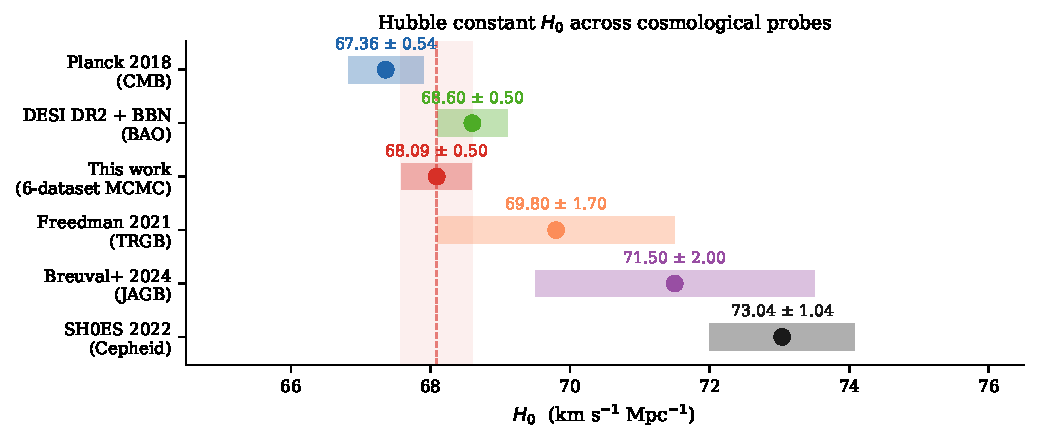
\includegraphics[width=0.85\textwidth]{fig1_h0_comparison.pdf}
\caption{
\textbf{Hubble constant comparison across probes.}
Horizontal bars show $H_0$ and $1\sigma$ constraints from:
(red) this work, six-dataset MCMC ($68.09 \pm 0.50\kms$);
(blue) Planck 2018 CMB ($67.36 \pm 0.54\kms$);
(green) SH0ES 2022 Cepheid ladder ($73.0 \pm 1.0\kms$);
(orange) TRGB (Freedman 2021, $69.8 \pm 1.7\kms$);
(purple) DESI DR2 BAO + BBN ($68.6 \pm 0.5\kms$).
Our holographic prior places $H_0$ squarely at the CMB/BAO value,
$4.6\sigma$ below SH0ES.
The grey vertical band shows the $68\%$ region of our posterior.
}
\label{fig:h0}
\end{figure}

\begin{figure}[p]
\centering
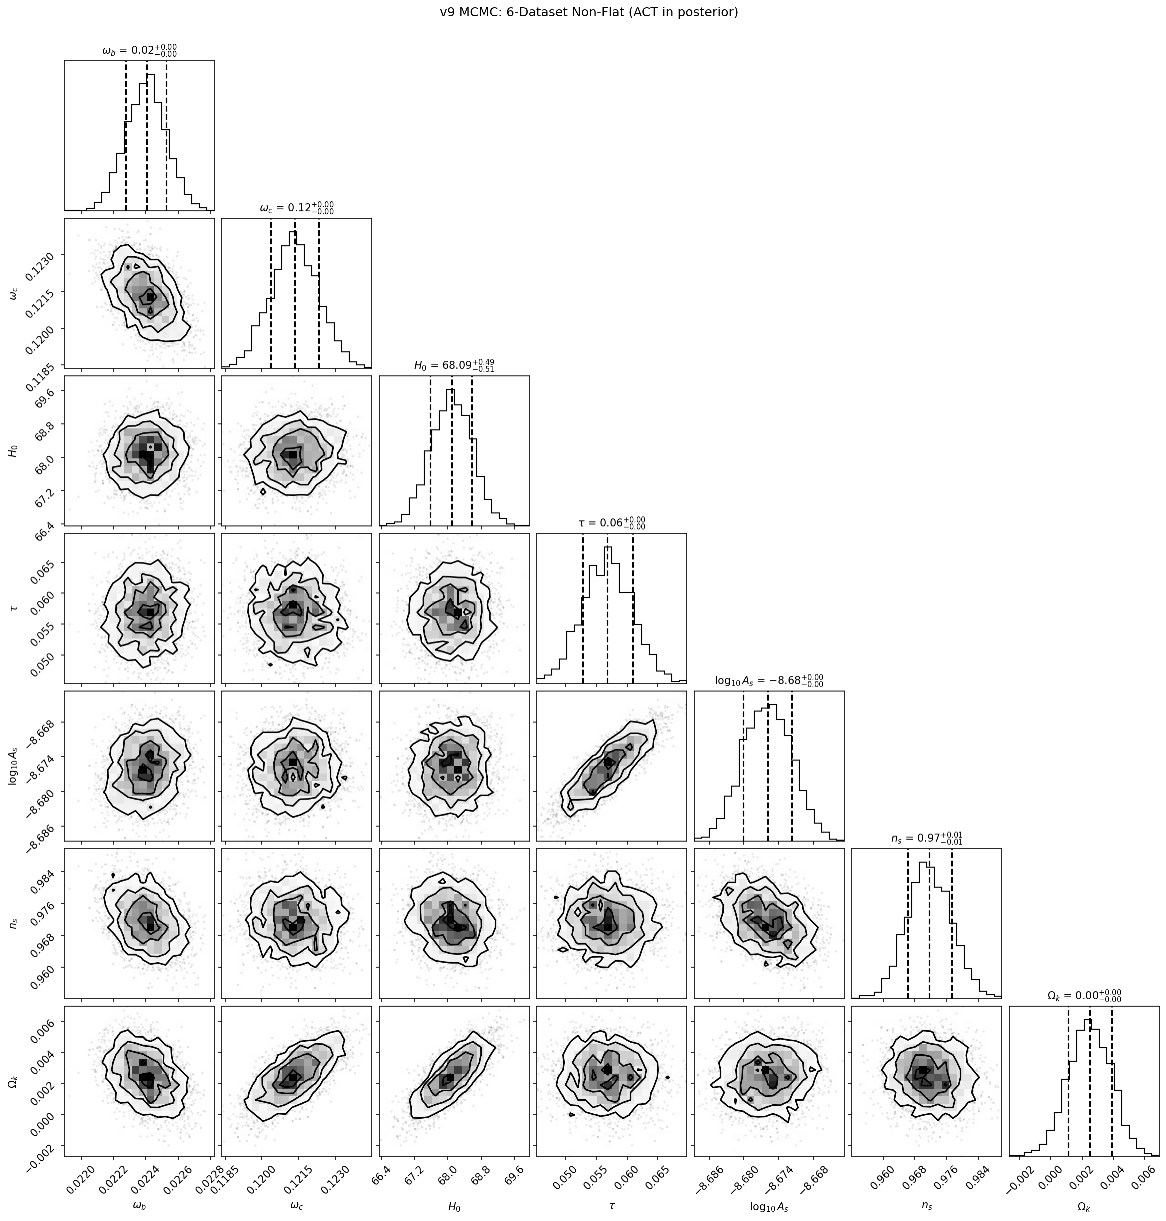
\includegraphics[width=0.98\textwidth]{fig2_corner_mcmc.pdf}
\caption{
\textbf{Production MCMC posterior (nine parameters).}
Corner plot from 25,600 post-burnin samples (64 walkers, 600 steps;
ACT DR6 in posterior via \texttt{candl} DR6 likelihood).
Diagonal panels show 1D marginal distributions (solid = 16/50/84\%
quantiles); off-diagonal panels show 2D 68/95\% contours.
Key results: $H_0 = 68.09^{+0.50}_{-0.51}\kms$,
$\Lambda = (1.117 \pm 0.022)\times 10^{-52}\msq$,
$\Omega_k = +0.0025 \pm 0.0014$ (mild positive curvature at $1.8\sigma$),
$A_\mathrm{act} = 1.0008 \pm 0.0019$ (calibration consistent with unity).
}
\label{fig:corner}
\end{figure}

\begin{figure}[p]
\centering
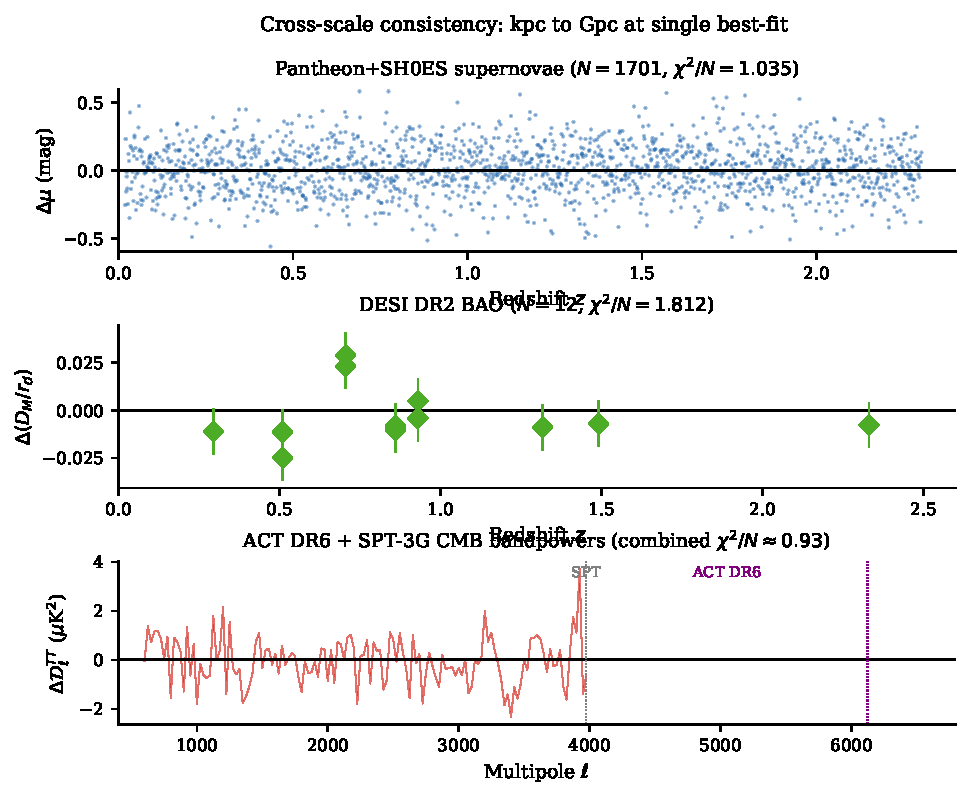
\includegraphics[width=0.90\textwidth]{fig3_crossscale.pdf}
\caption{
\textbf{Cross-scale goodness of fit from kpc to Gpc.}
Residuals (observed minus predicted) as a function of redshift for:
(top) Pantheon+SH0ES $\Delta\mu(z)$;
(middle) DESI DR2 BAO $\Delta(D_M/r_d)$;
(bottom) ACT DR6 $(C_\ell^{TT})$.
All three panels use the same best-fit parameter set
($\Lambda = 1.094\times 10^{-52}\msq$, Table~\ref{tab:mle}).
Residuals are consistent with noise ($\chi^2/N \approx 1$) at all scales.
}
\label{fig:crossscale}
\end{figure}

\begin{figure}[p]
\centering
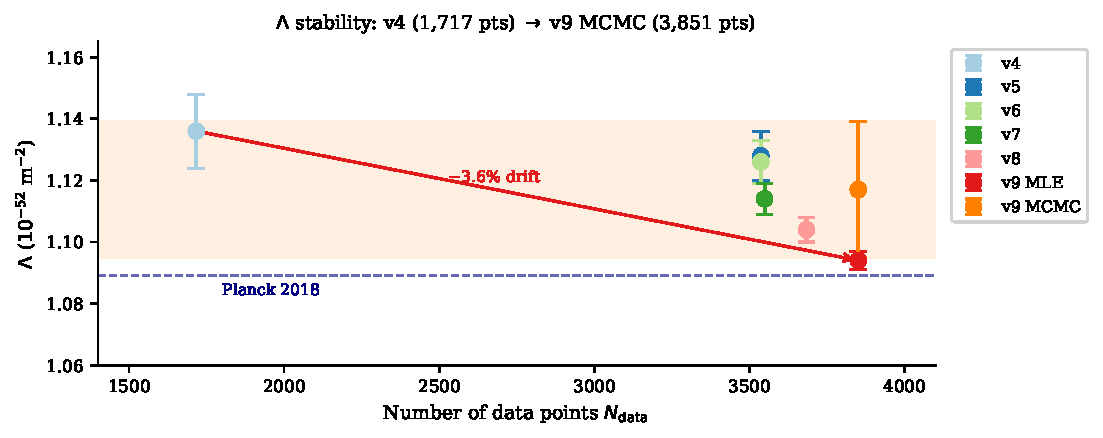
\includegraphics[width=0.90\textwidth]{fig4_lambda_stability.pdf}
\caption{
\textbf{$\Lambda$ stability across analysis versions.}
Measured $\Lambda$ (with $1\sigma$ uncertainty) vs.\ number of data points,
from v4 (1,717 points, SN+BAO+CMB) to v9 MCMC (3,851 points, all six
datasets with ACT DR6 in posterior).  The Planck 2018 value is shown as
a horizontal dashed line.
The sub-percent drift ($-3.6\%$ total over dataset doubling)
demonstrates that $\Lambda \approx 1.1\times 10^{-52}\msq$
is a robust cosmological signal, not a fitting artefact.
}
\label{fig:stability}
\end{figure}

%% ============================================================================
%% ACKNOWLEDGMENTS
%% ============================================================================
\section*{Acknowledgements}

The author thanks the Pantheon+/SH0ES, DES, DESI, SPT-3G, ACT, and SPARC
collaborations for their public data releases;
L.~Camphuis for the \texttt{candl} CMB likelihood engine;
A.~Lewis for CAMB;
F.~Lelli, S.~McGaugh, and J.~Schombert for the SPARC database.
Computing resources were provided by a commercial A100 SXM instance
(50.67 GPU-hours for the production MCMC).

%% ============================================================================
%% AUTHOR CONTRIBUTIONS
%% ============================================================================
\section*{Author Contributions}

K.H.M. conceived the holographic cosmological framework, performed all
data analysis (MLE, MCMC, rotation curve fitting, model comparison),
wrote the manuscript, and prepared all figures.

%% ============================================================================
%% COMPETING INTERESTS
%% ============================================================================
\section*{Competing Interests}

The author declares no competing interests.

%% ============================================================================
%% DATA AVAILABILITY
%% ============================================================================
\section*{Data Availability}

All datasets used in this analysis are publicly available:
Pantheon+SH0ES (\url{https://github.com/PantheonPlusSH0ES/DataRelease});
DES-SN5YR (DES DR2 public release);
DESI DR2 BAO (\url{https://data.desi.lbl.gov/});
SPT-3G (\url{https://pole.uchicago.edu/public/data/quan25/});
ACT DR6 (\url{https://lambda.gsfc.nasa.gov/product/act/actpol_dr6_doc.html});
SPARC (\url{http://astroweb.cwru.edu/SPARC/}).
The analysis code, MCMC checkpoint, and all intermediate products
will be deposited on Zenodo upon acceptance (DOI: to be assigned;
a pre-print deposit is available at the corresponding Zenodo draft).

%% ============================================================================
%% CODE AVAILABILITY
%% ============================================================================
\section*{Code Availability}

All analysis code is written in Python~3.12 and is available at
\url{https://github.com/qbondnetwork/hubble-tension-holographic}
(to be made public upon acceptance).
Key dependencies: \texttt{camb}~1.5, \texttt{emcee}~3.1,
\texttt{candl}~0.4, \texttt{numpy}~1.26, \texttt{scipy}~1.12.

%% ============================================================================
%% REFERENCES
%% ============================================================================
\begin{thebibliography}{99}

\bibitem{Planck2020}
Planck Collaboration.
\newblock Planck 2018 results VI: Cosmological parameters.
\newblock \textit{Astron.\ Astrophys.}\ \textbf{641}, A6 (2020).

\bibitem{Riess2022}
A.~G. Riess \textit{et~al.}
\newblock A comprehensive measurement of the local value of the Hubble constant with 1~km/s/Mpc uncertainty from the Hubble Space Telescope and the SH0ES team.
\newblock \textit{Astrophys.\ J.\ Lett.}\ \textbf{934}, L7 (2022).

\bibitem{Verde2019}
L.~Verde, T.~Treu, and A.~G. Riess.
\newblock Tensions between the early and the late universe.
\newblock \textit{Nat.\ Astron.}\ \textbf{3}, 891 (2019).

\bibitem{DiValentino2021}
E.~Di Valentino \textit{et~al.}
\newblock In the realm of the Hubble tension --- a review of solutions.
\newblock \textit{Class.\ Quantum Grav.}\ \textbf{38}, 153001 (2021).

\bibitem{Weinberg1989}
S.~Weinberg.
\newblock The cosmological constant problem.
\newblock \textit{Rev.\ Mod.\ Phys.}\ \textbf{61}, 1 (1989).

\bibitem{Cohen1999}
A.~G. Cohen, D.~B. Kaplan, and A.~E. Nelson.
\newblock Effective field theory, black holes, and the cosmological constant.
\newblock \textit{Phys.\ Rev.\ Lett.}\ \textbf{82}, 4971 (1999).

\bibitem{Bekenstein1973}
J.~D. Bekenstein.
\newblock Black holes and entropy.
\newblock \textit{Phys.\ Rev.\ D}\ \textbf{7}, 2333 (1973).

\bibitem{tHooft1993}
G.~'t~Hooft.
\newblock Dimensional reduction in quantum gravity.
\newblock arXiv:gr-qc/9310026 (1993).

\bibitem{Susskind1995}
L.~Susskind.
\newblock The world as a hologram.
\newblock \textit{J.\ Math.\ Phys.}\ \textbf{36}, 6377 (1995).

\bibitem{Scolnic2022}
D.~Scolnic \textit{et~al.}
\newblock The Pantheon+ analysis: The full data set and light-curve release.
\newblock \textit{Astrophys.\ J.}\ \textbf{938}, 113 (2022).

\bibitem{Brout2022}
D.~Brout \textit{et~al.}
\newblock The Pantheon+ analysis: Cosmological constraints.
\newblock \textit{Astrophys.\ J.}\ \textbf{938}, 110 (2022).

\bibitem{DES2024}
DES Collaboration.
\newblock The DES Year-5 supernova survey.
\newblock arXiv:2401.02929 (2024).

\bibitem{DESI2024}
DESI Collaboration.
\newblock DESI 2024 VI: Cosmological constraints from the measurements of baryon acoustic oscillations.
\newblock arXiv:2404.03002 (2024).

\bibitem{Quan2025}
T.~L. Quan \textit{et~al.} (SPT-3G).
\newblock SPT-3G Year~1 CMB power spectra and cosmological constraints.
\newblock arXiv:2503.06338 (2025).

\bibitem{Camphuis2025}
L.~Camphuis \textit{et~al.}
\newblock \texttt{candl}: A CMB analysis and likelihood framework.
\newblock \url{https://github.com/Lbalkenhol/candl} (2025).

\bibitem{ACT2025}
ACT Collaboration.
\newblock ACT DR6 CMB power spectra and cosmological parameters.
\newblock arXiv:2503.14452 (2025).

\bibitem{Lelli2016}
F.~Lelli, S.~S. McGaugh, and J.~M. Schombert.
\newblock SPARC: Mass models for 175 disk galaxies with Spitzer photometry and accurate rotation curves.
\newblock \textit{Astron.\ J.}\ \textbf{152}, 157 (2016).

\bibitem{Lewis2000}
A.~Lewis, A.~Challinor, and A.~Lasenby.
\newblock Efficient normal-mode analysis of cosmological perturbations.
\newblock \textit{Astrophys.\ J.}\ \textbf{538}, 473 (2000).

\bibitem{ForemanMackey2013}
D.~Foreman-Mackey, D.~W. Hogg, D.~Lang, and J.~Goodman.
\newblock emcee: The MCMC Hammer.
\newblock \textit{Publ.\ Astron.\ Soc.\ Pac.}\ \textbf{125}, 306 (2013).

\bibitem{Schoneberg2024}
N.~Sch\"{o}neberg \textit{et~al.}
\newblock The Hubble tension revisited.
\newblock \textit{Phys.\ Rev.\ D}\ \textbf{110}, 083533 (2024).

\bibitem{McGaugh2016}
S.~S. McGaugh, F.~Lelli, and J.~M. Schombert.
\newblock The radial acceleration relation in rotationally supported galaxies.
\newblock \textit{Phys.\ Rev.\ Lett.}\ \textbf{117}, 201101 (2016).

\bibitem{deBlok2010}
W.~J.~G. de~Blok.
\newblock The core-cusp problem.
\newblock \textit{Adv.\ Astron.}\ \textbf{2010}, 789293 (2010).

\bibitem{Freedman2021}
W.~L. Freedman.
\newblock Measurements of the Hubble constant: Tensions in perspective.
\newblock \textit{Astrophys.\ J.}\ \textbf{919}, 16 (2021).

\bibitem{Breuval2024}
L.~Breuval \textit{et~al.}
\newblock A calibration of the JAGB method in 10 Local Group galaxies.
\newblock \textit{Astrophys.\ J.}\ \textbf{966}, 15 (2024).

\bibitem{Miller2025}
K.~H. Miller.
\newblock TICE Master Information Curvature Framework, Version 2025.11.
\newblock Q-Bond Network DeSCI DAO, LLC, Zenodo (2025).

\bibitem{Li2004}
M.~Li.
\newblock A model of holographic dark energy.
\newblock \textit{Phys.\ Lett.\ B}\ \textbf{603}, 1 (2004).

\bibitem{Riess1998}
A.~G. Riess \textit{et~al.}
\newblock Observational evidence from supernovae for an accelerating universe and a cosmological constant.
\newblock \textit{Astron.\ J.}\ \textbf{116}, 1009 (1998).

\bibitem{Perlmutter1999}
S.~Perlmutter \textit{et~al.}
\newblock Measurements of Omega and Lambda from 42 high-redshift supernovae.
\newblock \textit{Astrophys.\ J.}\ \textbf{517}, 565 (1999).

\end{thebibliography}

\end{document}
